\documentclass[11pt]{article}
\usepackage[scaled=0.92]{helvet}
\usepackage{geometry}
\geometry{letterpaper,tmargin=1in,bmargin=1in,lmargin=1in,rmargin=1in}
\usepackage[parfill]{parskip} % Activate to begin paragraphs with an empty line rather than an indent %\usepackage{graphicx}
\usepackage{amsmath,amssymb, mathrsfs, dsfont}
\usepackage{tabularx}
\usepackage[font=footnotesize,labelfont=bf]{caption}
\usepackage{graphicx}
\usepackage{xcolor}
%\usepackage[linkbordercolor ={1 1 1} ]{hyperref}
%\usepackage[sf]{titlesec}
\usepackage{natbib}
\usepackage{../../Tianpei_Report}
%\usepackage{appendix}
%\usepackage{algorithm}
%\usepackage{algorithmic}

%\renewcommand{\algorithmicrequire}{\textbf{Input:}}
%\renewcommand{\algorithmicensure}{\textbf{Output:}}



\begin{document}
\title{Evaluation metrics for classification}
\author{ Tianpei Xie}
\date{Sep. 1st., 2022 }
\maketitle
\tableofcontents
\newpage
\allowdisplaybreaks
\section{Confusion table and related metrics}
\begin{itemize}
\item For a test set $T$ of examples and a classifier $f$, the \textbf{confusion matrix} \citep{japkowicz2011evaluating} $\mb{C}(f)$ can be defined as
\begin{align}
\mb{C}(f) = \set{c_{i.j}(f ) = \sum_{\mb{x} \in T}\ind{(y = i) \land (f(\mb{x}) = j)}} \in \bR^{l \times l},
\end{align} where $\mb{x}$ is a test example and $y$ is its corresponding label such that $y \in \{1, 2, \ldots, l\}$. Each element $c_{i,j}(f)$ of the confusion matrix denotes the number of examples that \emph{actually} have a class $i$ label and that the classifier $f$ \emph{assigns} to class $j$. Columns corespond to predicted values and rows correspond to true values. 

\item row sum $\sum_{j}c_{i,j}(f) = c_{i,\cdot}(f)$ denotes the total number of examples of class $i$ in the test set.
column sum $\sum_{i}c_{i,j}(f) = c_{\cdot,j}(f)$ denotes the total of examples assigned to class $j$ by classifier $f$.
diagonal sum is the total number of \emph{corrected classified} examples; all the nondiagonal entries denote \emph{misclassifications}.

\begin{figure}
\begin{minipage}[t]{1\linewidth}
  \centering
  \centerline{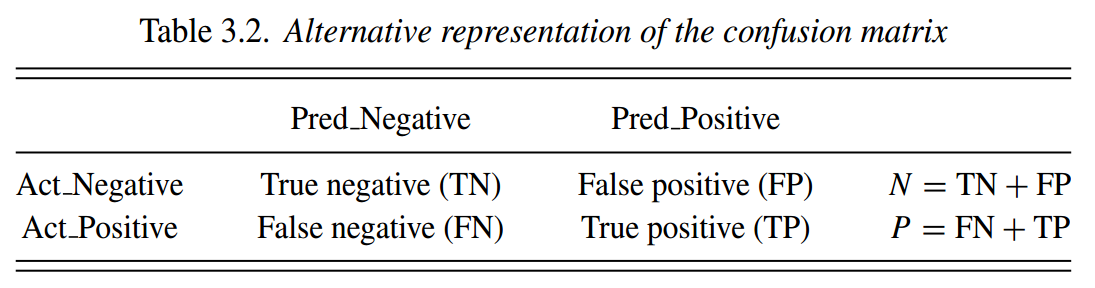
\includegraphics[scale = 0.35]{confusion_tab.png}}
\end{minipage}
\caption{\footnotesize{\textbf{The confusion table for binary classification}}}
\label{fig: confusion_tab}
\end{figure}

\item The \textbf{\emph{empirical error rate}} for classifier $f$ is 
\begin{align}
Error(f) &:= \frac{ \sum_{i \neq j} c_{i.j}(f) }{\sum_i \sum_{j} c_{i.j}(f) } \label{eqn: error_rate}
\end{align}


\item For binary classification, the confusion table looks as in Figure \ref{fig: confusion_tab}. Specifically, we define
\begin{itemize}
\item \textbf{True Positive (TP)} $\#\set{y=\text{positive}  \land  f(\mb{x}) = \text{positive}} = c_{1,1}(f)$;
\item \textbf{False Positive (FP)} $\#\set{y=\text{negative} \land  f(\mb{x}) = \text{positive} } = c_{0,1}(f)$;
\item \textbf{True Negative (TN)} $\#\set{y=\text{negative}  \land  f(\mb{x}) = \text{negative}} = c_{0,0}(f)$;
\item \textbf{False Negative (FN)} $\#\set{y=\text{positive} \land f(\mb{x}) = \text{negative} } = c_{1,0}(f)$;
\end{itemize} Total positives $= TP + FN$ and total negatives $=FP + TN$.

\item Given binary classficiation confusion table, define the followings
\begin{itemize}
\item \textbf{True Positive Rate (TPR)}: True positive among \emph{\textbf{all positives}} 
\begin{align}
\text{TPR}_{i} &= \frac{\text{TP}}{\text{TP}+ \text{FN}} = \frac{c_{i,i}(f)}{ \sum_{j} c_{i,j}(f) }. \label{eqn: tpr}
\end{align}  In its general form, this measure refers to the proportion of the examples of some class $i$ of interest actually assigned to class $i$ by the learning algorithm.

\item \textbf{False Positive Rate (FPR)}: False positive among \underline{\emph{\textbf{all negatives}}}
\begin{align}
\text{FPR}_{i} &= \frac{\text{FP}}{\text{FP} + \text{TN}} = \frac{\sum_{j\neq i} c_{j,i}(f)}{ \sum_{j\neq i}\sum_{k} c_{j,k}(f) }. \label{eqn: fpr}
\end{align} Note the denominator is \textbf{all negatives} not all positives.  FPRi(f ) measures the proportion of examples not belonging to class $i$
that are nonetheless erroneously classified as belonging to class $i$.

True- and false-positive rates generally form a \textbf{complement pair} of reported performance measures when the performance is \textit{measured over the} \underline{\emph{\textbf{positive}} class}
in the binary classification scenario.  Moreover, we can obtain the same measures on the \underline{\emph{negative} class} as below.

\item \textbf{True Negative Rate (TNR)}L True negatives among \emph{\textbf{all negatives}} 
\begin{align}
\text{TNR} &= \frac{\text{TN}}{\text{FP} + \text{TN}}. \label{eqn: tnr}
\end{align}
\item \textbf{False Negative Rate (FNR)}: False negatives among \underline{\emph{\textbf{all positives}}}. 
\begin{align}
\text{FNR} &= \frac{\text{FN}}{\text{TP} + \text{FN}}. \label{eqn: tnr}
\end{align} Note the denominator is \textbf{all positives} not all negatives. 

\item In signal detection theory, the true-positive rate is also known as the \emph{\textbf{hit rate}}, whereas the false-positive rate is referred to as the \emph{\textbf{false-alarm rate}} or the
\emph{fallout}. 
\end{itemize}

\item In hypothesis testing, with null hypothesis $\Theta_0$. The \textbf{\emph{type-I error}} $\alpha$ of test $T$ is 
\begin{align}
\alpha := \text{\textbf{type-I error}}(T) &= \bP\set{T(\mb{x}) \text{ \textbf{rejects} }\Theta_0 \;|\; \Theta_{0} \text{ is true}} \label{eqn: type-i_error}
\end{align} \underline{\textbf{FPR $=$ Type-I error}} when the null hypothesis $\Theta_0$ is \emph{\textbf{negative}}.

Similarly, the \emph{\textbf{type-II error}} $\beta$ of test $T$ is 
\begin{align}
\beta:= \text{\textbf{type-II error}}(T) &= \bP\set{T(\mb{x}) \text{ \textbf{failes to reject} }\Theta_0 \;|\; \Theta_{0} \text{ is false}} \label{eqn: type-ii_error}
\end{align} \underline{\textbf{FNR $=$ Type-II error}} when the null hypothesis $\Theta_0$ is \emph{\textbf{negative}}.

\item The true-positive rate of a classifier is also referred to as the \textbf{\emph{sensitivity}} of the classifier. For instance, it is used when investigating how sensitive the test is to the presence of the disease. The complement metric to this, in the case of the two-class scenario, would focus on the \emph{proportion of \textbf{negative} instances} (e.g., control cases or healthy subjects) that are detected. This metric is called the \emph{\textbf{specificity}} of the learning algorithm. 
\begin{itemize}
\item \textbf{\emph{sensitivity}} is defined as
\begin{align}
\text{sensitivity} &=  \frac{\text{TP}}{\text{TP}+ \text{FN}} =\text{TPR} \label{eqn: sensitivity}
\end{align}

\item \textbf{\emph{specificity}} is defined as
\begin{align}
\text{specificity} &= \frac{\text{TN}}{\text{FP} + \text{TN}} = \text{TNR} = (1- \text{FPR}) \label{eqn: specificity}
\end{align}
\end{itemize}

\item An important measure related to the sensitivity and specificity of the classifier, known as the \emph{\textbf{likelihood ratio}}, aims to combine these two notions to assess the extent to which the classifier is effective in predicting the two classes. Note the ratio is the likelihood of a given test result \emph{\textbf{under null hypothesis}} vs. the same test result \textit{\textbf{under alternative hypothesis}}. 
\begin{align}
\text{LR}_{+} &= \frac{\text{sensitivity} }{1 - \text{specificity}} \label{eqn: likelihood_ratio_pos}\\
\text{LR}_{-} &= \frac{1 -\text{sensitivity} }{\text{specificity}} \label{eqn: likelihood_ratio_pos}
\end{align} In terms of probabilities, LR$+$ is the ratio of the probability of a positive result in people who do encounter a recurrence to the probability of a positive
result in people who do not. Similarly, LR$-$ is the ratio of the probability of a negative result in people who do encounter a recurrence to the probability of a negative result in people who do not. 

A higher positive likelihood and a lower negative likelihood mean better performance on positive and negative classes, respectively, so we want to \emph{\textbf{maximize}} LR$+$ and \emph{\textbf{minimize}} LR$-$. 


\item Another aspect of assessment is the question of \emph{what the \textbf{proportion} of examples that \textbf{truly belong} to class $i$ is from among all the examples \textbf{assigned} to (or classified as) class $i$}.  We referred to it as \emph{\textbf{precision}} of a test:
\begin{align}
\text{PPV}(f)  = \text{Precision}(f) &= \frac{\text{TP}}{\text{TP} + \text{FP}} = \frac{c_{i,i}(f)}{\sum_{j}c_{j,i}(f)} =  \frac{c_{i,i}(f)}{c_{\cdot,i}(f)}  \label{eqn: precision}
\end{align} That is, this metric measures how "precise" the algorithm is when identifying the examples of a given class. It is also called \emph{\textbf{positive predictive value (PPV)}}.

Note that \textbf{\underline{precision is not equal to true positive rate,} nor false positive rate, false negative rate, true negative rate}. The TPR, FNR both assumed positive ground truth, while FPR, TNR assumes negative ground truth. However, the precision/PPV do not make assumption on fixed ground truth, instead focusing on the \emph{postive prediction} itself. One is conditioned on $y$, another one is conditioned on $f(\mb{x})$.

The counterpart of PPV in the binary classification scenario is the \emph{\textbf{negative predictive value (NPV)}}. PPV in this case typically refers to the class of interest (positive) whereas NPV measures the same quantity with respect to the negative (e.g., control experiments in medical applications) class.

A concrete judgment call on the superiority of the classifier in one case or the other is almost impossible based on the two metrics of PPV and NPV alone.   On the other
hand, with a reliability perspective, these metrics give an insight into how \underline{\textbf{\emph{reliable}}} the class-wise predictions of a classifier is.

\item \textbf{False discovery rate (FDR)} $\text{FDR} = \frac{\text{FP}}{\text{TP} + \text{FP}} = 1 - \text{PPV}$.

\item In information retrieval, we introduce the term "\emph{\textbf{recall}}", which is the TPR or sensitivity itself
\begin{align}
\text{Recall}(f) &= \text{TPR} = \text{sensitivity} =  \frac{\text{TP}}{\text{TP}+ \text{FN}}  \label{eqn: recall}
\end{align} So \underline{\textbf{recall is equal to true positive rate and is equal to sensitivity}}.

The pair $(\text{\textbf{PPV}}, \text{\textbf{TPR}}) = (\text{\textbf{Precision}}, \text{\textbf{Recall}})$ are typical statistics of interest in domains such as information retrieval in which we are interested not only in the \textit{\textbf{proportion of relevant information}} identified, but also in investigating the \textbf{actually relevant information} from the information \textbf{\emph{tagged as relevant}}. 

\item The \emph{F measure} attempts to address the issue of convenience brought on by a single metric versus a pair of metrics. It combines precision and recall in a single metric. More specifically, the \emph{\textbf{F measure}} is a \emph{weighted harmonic mean} of precision and recall. For any $\alpha \in \bR, \alpha > 0$, a general formulation of the F measure can be given as
\begin{align}
F_{\alpha} &=\frac{(1 + \alpha)\brac{\text{Precision}(f) \times \text{Recall}(f)}}{\brac{\alpha \times \text{Precision}(f)}+ \text{Recall}(f)}\nonumber\\
F_{1} &=  \frac{2 \brac{\text{Precision}(f) \times \text{Recall}(f)}}{\text{Precision}(f)+ \text{Recall}(f)}  \label{eqn: f_measure}
\end{align}

%\item Precision and recall are single-value metrics based on the whole list of documents returned by the system. For systems that return a ranked sequence of documents, it is desirable to also consider \textbf{\emph{the order}} in which the returned documents are presented. By computing a precision and recall \emph{at every position} in the \emph{\textbf{ranked sequence}} of documents, one can plot a precision-recall curve, plotting precision as a function of recall $r$.

\item \textbf{\emph{Precision at $k$}} (referred as $P@k$) is the precision value among \underline{\emph{top $k$ retrieval results}}. Its shortcoming is thatit  fails to take into account the positions of the relevant documents among the top $k$.

\item  \textbf{\emph{Average precision}} computes the average value of $p(r)$ over the interval from recall $r=0$ to $r=1$:
\begin{align}
\text{AveP} &= \int_0^{1}p(r) dr = \frac{\sum_{k=1}^{n}\text{Precision}(k)\,\ind{d_k \text{ at rank }k \text{ is relevent}}}{\#\text{ relevent docs}} \label{eqn: average_precision}
\end{align} It is the \underline{\emph{\textbf{area under PR-curve}} (AUC of PR)}. $\text{Precision}(k)$ is the precision at cut-off rank $k$ in the list. 

\item The \emph{\textbf{interpolated precision}} $p_{\text{interp}}$ at \emph{a certain \textbf{recall} level} $r$ is defined as the highest precision found for any recall level $r' \ge r$:
\begin{align}
p_{\text{interp}}(r)&:= \max_{r' \ge r}p(r')  \label{eqn: interpolated_precision}
\end{align} Some choose \emph{\textbf{$11$-point interpolated average precisio}n} $\text{AveP} = \frac{1}{11}\sum_{r \in \{0, 0.1,\ldots, 1.0 \} }p_{\text{interp}}(r)$.


\item \emph{\textbf{Mean average precision (MAP)}} for a set of queries is the \emph{mean} of the \emph{average precision} scores for \emph{\textbf{each query}} \citep{manning2008introduction}.
\begin{align}
\text{MAP} &= \frac{1}{Q}\sum_{q=1}^{Q}\text{AveP}(q) \label{eqn: mean_average_precision}
\end{align}
\end{itemize}

\section{Receiver Operating Characteristic (ROC)}
\subsection{Graphical Performance Measures}
It is desirable for a performance measure not only to take into account the information contained in the confusion matrix, but also to incorporate considerations such as \emph{skew} and \emph{prior class distributions}. Moreover, when dealing with a scoring classifier, it is often desirable that the measure enables an assessment of classifier performance over its full operating range (of possible scores).   Typically, information related to skew, cost, or prior probabilities (other than the class distribution in the training set) of the data is generally not known. Even when the asymmetric nature of the misclassification cost is known, it is not easily quantifiable. Graphical performance measures are very useful in such cases because they enable visualization of the classifier performance over the full operating range and hence under different skew ratios and class distribution priors.

Graphical performance measures has advantages when we want to discover zones of optimality, given the information over the full operating range. The question
of choosing one single optimal classifier based on some quantification of the resulting graphs gives rise to measures that incorporate all the details into a scalar metric. Inevitably, compressing the information in a scalar metric results in significant information loss.
\begin{figure}
\begin{minipage}[t]{1\linewidth}
  \centering
  \centerline{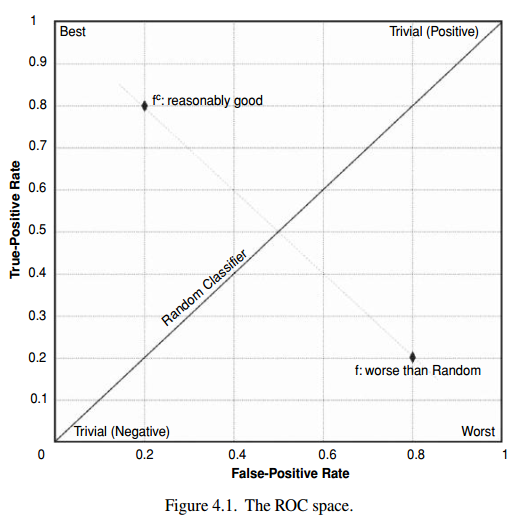
\includegraphics[scale = 0.5]{roc_curve.png}}
\end{minipage}
\caption{\footnotesize{\textbf{The ROC space}}}
\label{fig: roc_curve}
\end{figure}
\subsection{ROC Space}
\underline{\emph{\textbf{Receiver operating characteristic (ROC)}}} analysis has its origin in signal detection theory as a means to set a threshold or an operating point for the receiver to detect the presence or absence of signal. An \emph{\textbf{ROC curve}} is a plot in which the \textbf{horizontal axis} (the x axis) denotes the \emph{false-positive rate \textbf{FPR}} and the \textbf{vertical axis} (the y axis) denotes the \emph{true-positive rate \textbf{TPR}} of a classifier. 

Note that the \textbf{TPR $=$ sensitivity} of the classifier whereas the \textbf{FPR $=$ $1-$TNR} (TNR is the true negative rate) or equivalently
$1 –$ specificity of the classifier. Hence, in this sense, \emph{\textbf{ROC analysis} studies the relationship between the \textbf{sensitivity} and the \textbf{specificity} of the classifier}. (It is like likelihood rato $\text{LR}_{+}$)

Because, for both the TPR and FPR, it holds that $0 \le \text{TPR} \le 1$ and $0 \le \text{FPR} \le 1$, the ROC space is a unit square, as shown in Figure \ref{fig: roc_curve}. The output of a deterministic classifier results in a single point in this ROC space. The \underline{point $(0, 0)$} denotes a trivial classifier that \emph{classifies \textbf{all} the instances as \underline{\textbf{negative}}} and hence results in both the TPR and the FPR being zero. On the other end of the square, the \underline{point $(1, 1)$} corresponds to the trivial classifier that \emph{labels \textbf{all} the instances as \underline{\textbf{positive}}} and hence has both the TPR and the FPR values of unity.

The diagonal connecting these two points [(0, 0) and (1, 1)] has \underline{\textbf{TPR = FPR}} at all the points. The classifiers falling along this diagonal can hence be considered
to be \underline{\emph{\textbf{random classifiers}}} (that is, they assign positive and negative labels to the instances randomly). This resembles a biased coin toss at every point along the diagonal with bias $p = \text{TPR} = \text{FPR}$ of assigning a positive label and $1 - p$ of assigning a negative label. 

The points (1, 0) and (0, 1) give the other two extremes of the ROC space. The \underline{point (1, 0)} has FPR = 1 and TPR = 0, meaning that the classifier denoted by this point gets \emph{\textbf{all its predictions wrong}}. On the other hand, the \underline{point (0, 1)} denotes the ideal classifier, one that gets \emph{\textbf{all the positives right} and makes \textbf{no errors on the negatives}}. The diagonal connecting these two points has \underline{\textbf{TPR = 1 - FPR = TNR}}. This goes to show that the \emph{classifiers along this diagonal perform \textbf{equally well on both the positive and the negative classes}}.

An \underline{\emph{\textbf{operating point}}} in the ROC space corresponds to a particular \textbf{decision threshold} of the classifier that is used to assign discrete labels to the examples. As just mentioned, the instances achieving a score \emph{\textbf{above}} the threshold are labeled \emph{positive} whereas the ones \emph{below} are labeled \emph{negative}. \textbf{Each point} on the ROC space denotes a particular \textbf{TPR and FPR} for a classifier. Now,\emph{ each such point will have an associated confusion matrix} summarizing the classifier performance. Consequently an \textbf{ROC curve is a \underline{collection of various \emph{confusion matrices}} over different \emph{varying decision thresholds}} for a classifier.



Theoretically, we can obtaint the ROC curve by tuning the decision threshold over the continuous interval between the minimum and maximum scores received by the instances in the dataset. However, this is not necessarily the case in most practical scenarios. There are two reasons:
\begin{itemize}
\item The \textbf{limited size} of the dataset limits the number of values on the ROC curves that can be realized. That is, when the instances are \emph{\textbf{sorted}}
in terms of the \emph{\textbf{classification scores}}, then all the decision thresholds in the \underline{\emph{\textbf{interval of scores}}} of any \underline{\emph{\textbf{two consecutive instances}}} will essentially give the same TPR and FPR on the dataset, resulting \textbf{in a single point}. The maximum number of points that can be obtained are \textbf{upper bounded by} the \textbf{number of examples} in the dataset

\item This argument assumes that a \emph{\textbf{continuous tuning}} of the decision threshold is indeed possible. This is not necessarily the case for all the scoring classifiers. Classifiers such as \textbf{decision trees}, for instance, allow for only a finite number of thresholds (\textbf{upper bounded} by the number of \emph{possible labels} over the \emph{leafs of the decision tree}). 
\end{itemize}

Based on ROC curves, we can compare different classifiers.
\begin{itemize}
\item The classifiers appearing on the \underline{\textbf{left-hand side}} on an ROC graph can be thought of as more \underline{\emph{\textbf{conservative}}} in their classification of positive examples. They \textbf{demand \underline{\emph{low FPR}}},  \underline{\textbf{preferring misclassifying positive}} examples to risking the \textbf{misclassification of negative} examples.

\item The classifiers on the \underline{\textbf{right-hand side}}, on the other hand, are more \underline{\emph{\textbf{liberal}}} in their classification of positive examples, meaning that they \textbf{prefer misclassifying negative} examples \textbf{to failing to recognize a positive example} as such. 
\end{itemize} This can be seen as quite a useful feature of ROC graphs because different operating points might be desired in the context of different application settings.

Each point on the ROC curve represents a different \textbf{trade-off} between the \emph{false positives} and \emph{false negatives} (also known as \emph{\textbf{the cost ratio}}). The cost ratio is defined by the \textbf{slope} of the line \textbf{tangent to the ROC curve} at a given point.

\subsection{Skew Considerations}

The \emph{ROC graphs} are \underline{\textbf{\emph{insensitive to class skews (or class imbalances})}}. This is because ROC plots are measures of \textbf{TPR} and \textbf{FPR} of a classifier and do \textbf{not} take into account the actual class distributions of the positive and negative examples, unlike measures such as accuracy, empirical risk, or the F measure. 

However, this observation has both a significant underlying \textit{\textbf{assumption}} and subsequent implications. An ROC curve is based on a $2 \times 2$ confusion
matrix, which has $3$ degrees of freedom. The points in the \textbf{2D ROC space} hence are essentially \textbf{projections of points from a three-dimensional (3D) space}. The first two dimensions of the space correspond to the TPR and the FPR. However, the third dimension generally depends on the \emph{specific performance measure} used to evaluate the algorithm. We can add the \textbf{class-ratio as the third dimension}. This third dimension enables us to characterize the various TPRs and FPRs that can be realized by the classifier over its entire operating range and, further, \textbf{over different class distributions}.

When considering performances on a 2D slice of the 3D ROC space, we have the \emph{\textbf{implicit assumption}} that \textbf{TPR and the FPR are \underline{independent} of the empirical (or expected) class distributions}. 

More generally, the factors such as \emph{class imbalances}, \emph{misclassification costs}, and \emph{credits for correct classification} can be incorporated by a single metric, \emph{\textbf{the skew ratio}}. A skew ratio $r_s$ can be utilized such that $r_s < 1$ if positive examples are deemed more important, for instance, because of a class imbalance with fewer positives in the test set compared with the negatives or because of a high misclassification cost associated with the positives. 
\subsection{Isometrics}
\begin{figure}
\begin{minipage}[t]{1\linewidth}
  \centering
  \centerline{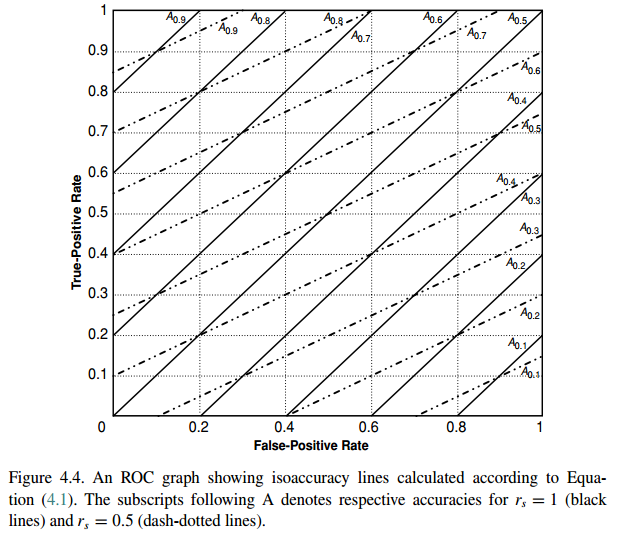
\includegraphics[scale = 0.5]{isoaccuracy.png}}
\end{minipage}
\begin{minipage}[t]{1\linewidth}
  \centering
  \centerline{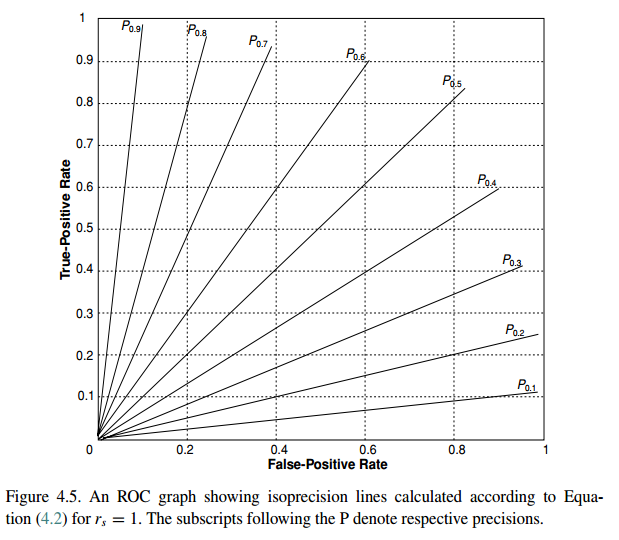
\includegraphics[scale = 0.5]{isoprecision.png}}
\end{minipage}
\caption{\footnotesize{\textbf{The isometrics for given skew ratio.}}}
\label{fig: isometrics}
\end{figure}


To select an optimal operating point on the ROC curve, any performance measure can be used as long as it can be formulated in terms of the algorithm’s TPR and FPR. For instance, given a skew ratio $r_s$ we can define the \emph{(skew-sensitive) formulation of the \underline{\textbf{accuracy}}} of classifier $f$ as
\begin{align}
\text{Acc}(f) &= \frac{\text{TPR}(f) + (1 - r_s) \text{FPR}(f) }{1 + r_s}\label{eqn: skew_accuracy}
\end{align} where $r_s$ is the skew ratio (class ratio)
\begin{align*}
r_s &= \frac{\text{FP} + \text{TN}}{\text{TP} + \text{FN}} = \frac{\#\text{N}}{\#\text{P}}
\end{align*}

Given the preceding definition of accuracy for a fixed $r_s$, the lines in the 2D ROC curve with the same value of accuracy are referred to as the \emph{isoaccuracy lines}. More generally, for any performance measure or metric, such lines or curves denoting the \textbf{same metric value} for a given $r_s$ are referred to as \emph{\textbf{isometrics}} or \emph{\textbf{isoperformances}} lines (or curves). 




We can also represent the \underline{\textbf{precision}} in terms of the algorithm’s TPR and FPR
\begin{align}
\text{Precision}(f) &= \frac{\text{TPR}(f)}{\text{TPR}(f) + r_{s}\,\text{FPR}(f)} \label{eqn: skew_precision}
\end{align} Under the preceding definition of rs, we can obtain isoprecision lines on the 2D
ROC graph (and surfaces in the 3D ROC space).

For a given performance measure, we can consider the \textbf{highest point} on the ROC curve that touches a given \textbf{isoperformance line} of interest (that is, with desired $r_s$) to select the desired operating point. This can be easily done by starting with the desired isoperformance line at the best classifier position in the
ROC graph \textbf{(FPR = 0, TPR = 1)} and gradually sliding it down until it touches one or more points on the curve. The points thus obtained are \emph{\textbf{the optimal
performances}} of the algorithm for a desired skew ratio. We can obtain the value of the performance measure at this optimal point by looking at the \emph{\textbf{intersection}} of the \textbf{isoperformance} line and the \textbf{diagonal} connecting the points (FPR = 0, TPR = 1) and (FPR = 1, TPR = 0). 

The line for isopermission and isoaccuracy is as below
\begin{align*}
 \text{TPR}(f) &= \frac{r_{s}\,\text{Precision}(f)}{(1-\text{Precision}(f)) }\,\text{FPR}(f) \\
 \text{TPR}(f) &= - (1 - r_s) \text{FPR}(f)  + (1 + r_s)\text{Acc}(f) 
\end{align*} See Figure \ref{fig: isometrics} for illustrations on isometrics.

The set of points on the ROC curve that are \emph{\textbf{not suboptimal}} forms the  \emph{\textbf{ROC convex hull (ROCCH)}}. The classifiers in
the convex hull represent the \emph{\textbf{optimal classifiers}} (under a given performance measure) for a given skew ratio. Moreover, in the case of multiple classifiers, the convex hull identifies the best classifier(s) for different operating points. The points on the ROC curve of a learning algorithm give a snapshot of the classifier performance for a given skew ratio. 


\subsection{ROC Curve Generation}
\begin{figure}
\begin{minipage}[t]{1\linewidth}
  \centering
  \centerline{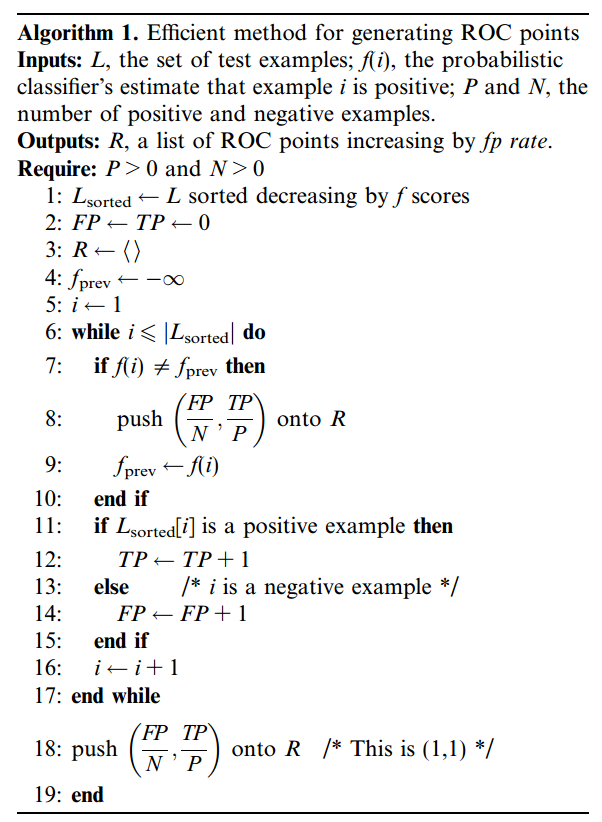
\includegraphics[scale = 0.45]{roc_generation.png}}
\end{minipage}
\caption{\footnotesize{\textbf{The algorithm to generate ROC curve \citep{fawcett2006introduction}}}}
\label{fig: roc_generation}
\end{figure}


The efficient implementations of the ROC curve-generation process can also be found as a standard package in many machine learning toolkits. We attached an efficient algorithm by \citep{fawcett2006introduction} in Figure \ref{fig: roc_generation}.


In the algorithm, we exploit the \underline{\emph{\textbf{monotonicity} of thresholded classifications}}: any instance that is classified \emph{positive} with respect to a given threshold will be classified \emph{positive} for \emph{\textbf{all lower thresholds}} as well. $y_{+} = f(x) \ge t_{0} \Rightarrow y_{+} = f(x) \ge t, \forall t \le t_{0}.$ We can simply \textbf{sort} the test instances \textbf{decreasing} by $f$ scores and move down the list, processing one instance at a time and updating TP and FP as we go. In this way an ROC graph can be created from a linear scan. Statements 7-10 need some explanation. These are necessary in order to correctly handle sequences of \emph{equally scored instances}. 

Let $n$ be the number of points in the test set. This algorithm requires an $O(n\log n)$ sort followed by an $O(n)$ scan down the list, \textbf{resulting in $O(n\log n)$ total complexity}.
\subsection{Summary Statistics and the AUC}



ROC curve does not allow us to quantify this comparative analysis that can facilitate decision making with regard to the suitability or preference of one classifier over others in the form of an objective \emph{\textbf{scalar metric}}. Some such representative statistics include these:
\begin{itemize}
\item The area \emph{\textbf{between}} the ROC curve and the diagonal of the ROC graph connecting the points FPR = TPR = 0 and FPR = TPR = 1; It measures the performance that a learning algorithm can achieve above the random classifier along TPR = FPR.
\item The \emph{\textbf{intercept}} of the ROC curve with the diagonal connecting FPR = 1, TPR = 0 and FPR = 0, TPR = 1; This statistics signifies
the \emph{operating range} of the algorithm that yields classifiers with \emph{lower expected cost}.
\item The \emph{\textbf{total area} under the ROC curve}, abbreviated as \emph{\textbf{AUC}}.
\end{itemize}

The \textbf{AUC} represents the performance of the classifier \underline{\emph{\textbf{averaged}} over \emph{all the possible cost ratios}}. $\text{AUC}(f) \in [0,1]$,  with the upper bound attained for a perfect classifier (one with TPR = 1 and FPR = 0).  The \emph{\textbf{random} classifier} represented by the diagonal cuts the ROC space in half and hence $\text{AUC}(f_{\text{random}}) = 0.5$. On the other hand, if the classifier assigns the \emph{\textbf{same score to all examples}}, whether \emph{negative} or \emph{positive}, we would obtain classifiers along the diagonal \textbf{TPR = FPR}. We can also obtain a similar curve if the classifier \emph{assigns similar distributions} of the score. 

\textbf{Another interpretation} of an \textbf{AUC} can be obtained for \underline{\textbf{ranking classifiers}} in that AUC represents the \textbf{ability} of a classifier to rank a \emph{randomly} chosen \textbf{positive} test example \textbf{higher than} a negative one. In this respect, this is shown to \textbf{be equivalent to} \underline{\textbf{\emph{Wilcoxon's Rank Sum test}}} (also known as the \emph{\textbf{Mann-Whitney U test}}).  With regard to the \emph{\textbf{Gini
coefficient (Gini)}}, a measure of statistical dispersion popular in economics, it has been shown that $$\text{AUC} = \frac{(Gini + 1)}{2}$$.

A simpler algorithm to estimate AUC is to use Wilcoxon’s Rank Sum statistic. We first \textbf{rank} the scores for each test instances \textbf{in decreasing order}. Then we can calculate the AUC as
\begin{align}
\text{AUC}(f) &= \frac{\sum_{i}^{|T_{p}|}(R_i - i)}{|T_{p}|\, |T_{n}|},  \label{eqn: auc_compute_wilcoxon}
\end{align} where $T_{p} \subset  T$  and $T_n \subset T$ are, respectively, the subsets of \emph{positive} and \emph{negative} examples in test set $T$ , and $R_i$ is the rank of the $i$-th example in $T_p$ given by classifier $f$. Computing AUC can be done simiar to computing ROC, which is $O(n \log n)$. 

As other single-metric performance measures, AUC misses  information on \emph{\textbf{concavities} in the performance}, or \textit{\textbf{trade-off behaviors}} between the true-positive and the false-positive performances. 

\begin{figure}
\begin{minipage}[t]{1\linewidth}
  \centering
  \centerline{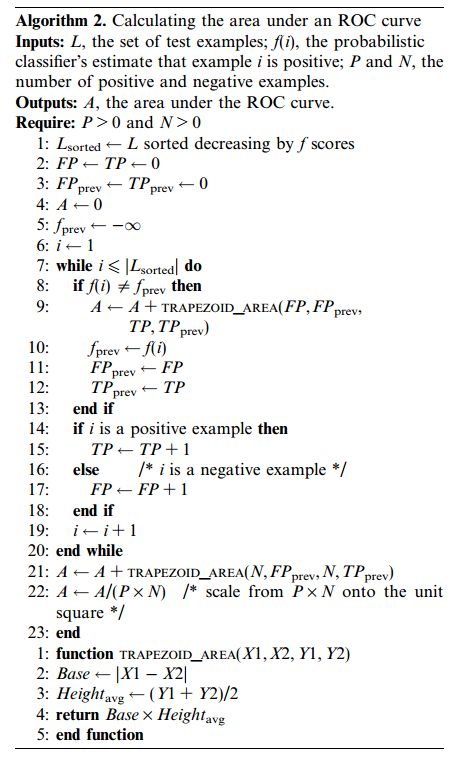
\includegraphics[scale = 0.5]{auc.png}}
\end{minipage}
\caption{\footnotesize{\textbf{The algorithm to compute AUC of ROC curve \citep{fawcett2006introduction}}}}
\label{fig: auc}
\end{figure}


Some criticisms have also appeared warning against the use of AUC across classifiers \textbf{for comparative purposes}. 
\begin{itemize}
\item One of the most obvious is that, because the classifiers
are typically optimized to obtain the best performance (in context of the given performance measure), the ROC curves thus obtained in the two cases would be similar. This then would yield \emph{uninformative AUC differences}.
\item Further, if the \textbf{ROC curves} of the two classifiers \textbf{\emph{intersect}}, the AUC-based comparison between the classifiers can be relativly uninformative and even \textbf{misleading}. 
\item  However, a more serious limitation of the AUC for
comparative purposes lies in the fact that the \emph{misclassification \textbf{cost} distributions} (and hence the \textbf{skew-ratio} distributions) used by the AUC are different for different classifiers. 
\end{itemize}

In the event the \textbf{\underline{\emph{ranking property}} of the classifier} is important (for instance, in information-retrieval systems), AUC can be a more reliable measure
of classifier performance than measures such as accuracy because it \textbf{assesses the ranking capability} of the classifier in a direct manner. 


\subsection{Calibration}
\begin{figure}
\begin{minipage}[t]{1\linewidth}
  \centering
  \centerline{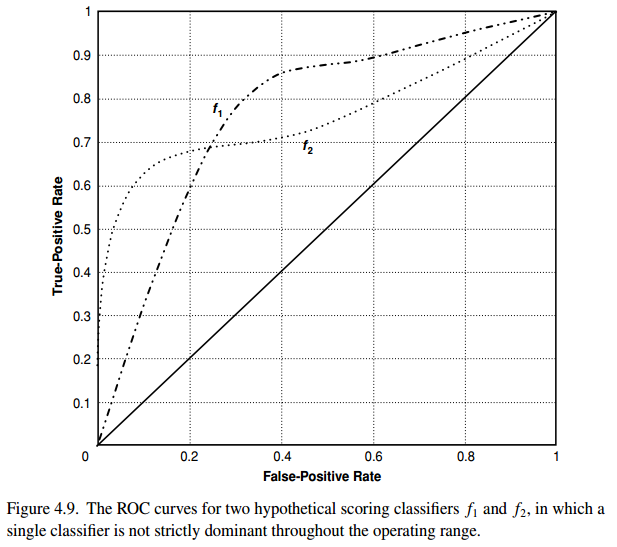
\includegraphics[scale = 0.5]{roc_two_classifiers.png}}
\end{minipage}
\caption{\footnotesize{\textbf{The comparison of two algorithms in ROC curve \citep{japkowicz2011evaluating}}}}
\label{fig: roc_two_classifiers}
\end{figure}

The classifiers' thresholds based on the training set may or may not reflect the empirical realizations of labelings in the test set. That is, if no example obtains a score in the interval $[t_1, t_2] \subset I$, then no threshold in the interval $[t_1, t_2]$ will yield a different point in the ROC space. One solution to deal with this problem is
\emph{\textbf{calibration}}. All the scores in the interval $[t_1, t_2]$ can be mapped to the fraction of the positive instances obtained as a result of assigning any score in this interval, i.e. \emph{linear interpolation}.

This is a workable solution as long as there are \emph{no \textbf{concavities} in the ROC curve}.  \textbf{Concavity} in the curve means that there are \emph{\textbf{skew ratios}} for which the classifier is \emph{\textbf{suboptimal}}. This essentially means that \textbf{better classifier}  performance can be obtained for the skew ratios lying in the \emph{concave region} of the curve although the empirical estimates do not suggest this. See Figure \ref{fig: roc_two_classifiers}. In the case of concavities, the behavior of the calibrated scores does not mimic the desired behavior of the slope of the threshold interval. The classifier obtained over \emph{\textbf{calibrated}} scores can \textbf{overfit} the data, resulting in poor generalization. One can use \textbf{isotonic regression} to map the scores corresponding to the \emph{concave interval} $[t_1, t_2]$  to an \emph{unbiased} estimate of the slope of the line segment connecting the two points corresponding to the thresholds $t_1$ and $t_2$.
\section{Other Visual Analysis Methods}
\subsection{Precision-Recall (PR) Curves}
\emph{\textbf{Precision-recall Curves}}, sometimes abbreviated as \emph{\textbf{PR curves}}, are similar to ROC curves and lift charts in that they explore the trade-off between the wellclassified positive examples and the number of misclassified negative examples. As the name suggests, PR curves plot the \textbf{precision} of the classifier as \textbf{a function of its recall}.  

The curves look \textbf{different} from ROC curves and lift curves because they have a \textbf{\emph{negative slope}}. This is because precision \textbf{decreases} as recall \textbf{increases}. PR  curves can sometimes be more appropriate than the ROC curves in the events of \emph{\textbf{highly imbalanced data}} \citep{davis2006relationship}.

\subsection{Lift Charts}
\textbf{\emph{Lift charts}} are a performance visualization technique closely related to the ROC curves. Lift charts plot the \underline{\textbf{true positives}} against the \textbf{dataset size} required to \textbf{achieve} this number of true positives. That is, the \emph{\textbf{vertical axis}} of the lift charts plots \textbf{\emph{the true positives}} (and \textbf{not the TPR}) whereas the \emph{\textbf{horizontal axis}} denotes the \textbf{number of examples} in the dataset considered for the specific true positives on the vertical axis. 

In other words, the ROC curve counts the number of negative examples that have slipped into the data sample for which the classifier issued
a particular true-positive rate, whereas the lift chart  \textbf{counts both the positive and the negative examples} in that set.  In \textbf{highly imbalanced datasets}, in which,
typically the number of positive examples is much smaller than that of negative examples, the horizontal axes of lift charts and ROC curves look \textbf{very similar} as do the curves.
\newpage
\bibliographystyle{plainnat}
\bibliography{book_reference.bib}
\end{document}